\documentclass[preprint,12pt]{elsarticle}
\usepackage{amsmath,amssymb,amsthm,booktabs,graphicx,xcolor}
\usepackage{xr-hyper}
\usepackage[hidelinks]{hyperref}
\externaldocument[][nocite]{sod_rom_v4_supp}
\usepackage{tikz}
\usepackage[subpreambles=true]{standalone}  % Fig. 1 is the TikZ file ../figures/tikz/fig_c_systems_tikz.tex
% shared macros for the SOD tutorial and papers
% Typesetting follows ISO 80000-2: italic scalars (capital Greek via \var...),
% bold italic vectors and matrices (\bm), upright d, e, i, operators and labels.
\usepackage{bm,upgreek}
\newcommand{\bx}{\bm{x}}  \newcommand{\bz}{\bm{z}}  \newcommand{\bX}{\bm{X}}
\newcommand{\bV}{\bm{V}}  \newcommand{\bW}{\bm{W}}  \newcommand{\bU}{\bm{U}}
\newcommand{\bM}{\bm{M}}  \newcommand{\bK}{\bm{K}}  \newcommand{\bC}{\bm{C}}
\newcommand{\bA}{\bm{A}}  \newcommand{\bB}{\bm{B}}  \newcommand{\bS}{\bm{S}}
\newcommand{\bI}{\bm{I}}  \newcommand{\bff}{\bm{f}}
\newcommand{\bSig}{\bm{\varSigma}}  \newcommand{\bpsi}{\bm{\psi}}  \newcommand{\bPsi}{\bm{\varPsi}}
\newcommand{\bphi}{\bm{\phi}}  \newcommand{\bPhi}{\bm{\varPhi}}
\newcommand{\avg}[1]{\left\langle #1 \right\rangle}
\newcommand{\bnd}[1]{\left[ #1 \right]_T}
\newcommand{\sym}{\operatorname{sym}}  \newcommand{\skw}{\operatorname{skew}}
\newcommand{\TODO}[2]{\textcolor{red}{\textbf{[#1]} #2}}

% scalars: A, E, H, I, L, P, R, T, W, \varOmega, \varGamma
% elsarticle appends a period to every \paragraph title; the titles here carry
% their own punctuation (some end in '?'), so the automatic period is removed.
\makeatletter
\def\els@aparagraph[#1]#2{\elsparagraph[#1]{#2}}
\def\els@bparagraph#1{\elsparagraph*{#1}}
\makeatother
\graphicspath{{../figures/}}
\newtheorem{proposition}{Proposition}
\setlength{\emergencystretch}{3em}
\journal{Journal of Sound and Vibration}
\begin{document}
\begin{frontmatter}
\title{Smooth orthogonal decomposition bases learn static correction from response records}
\author[nld]{David Chelidze}
\ead{chelidze@uri.edu}
\affiliation[nld]{organization={Nonlinear Dynamics Laboratory, Department of Mechanical, Industrial and Systems Engineering, University of Rhode Island},
            city={Kingston}, state={RI}, postcode={02881}, country={USA}}


\begin{abstract}
Smooth orthogonal decomposition (SOD) builds reduced-order model (ROM) bases from response records, without an eigensolution of the model. Earlier studies reported SOD ROMs more accurate than proper orthogonal decomposition and faster than the full model, without identifying which directions a data basis contains that a model-based basis lacks.
On a cantilever, one SOD basis trained on a random tip load is 27 times more accurate than the linear normal modes (LNMs) at eight modes, yet less accurate at three modes and under a mid-span load.
We test the hypothesis that the basis holds the directions its record visits: the quasi-static response of truncated modes at the loaded points, which static correction (modal truncation augmentation, MTA) adds from the model.
At eight modes the SOD subspace contains the static tip-load vector about 190 times better than the LNMs, and the mid-span one no better.
The obstacle is ranking: ordered by smoothness, the same quasi-static direction enters at the third mode and displaces a mode inside the load band.
Recognising modes by their own spectral peak, or by the one-way rotation of a modal plane, and placing them first removes the loss.
With the same load locations, SOD and MTA ROMs agreed within a factor of 3.4.
A local nonlinear force acts in a free decay, so one decay supplied its correction without its location. On two nonlinear cantilevers the first SOD direction lay within $0.05^\circ$ of the tip deflection under a harmonic tip force at the first SOD frequency. On the two-well cantilever MTA was more accurate from three modes on.
At matched integration accuracy, truncation lowered the cost; the SOD coordinates did not.
A data basis therefore needs a training record at every external load location, with the bandwidth and rank to contain the quasi-static response. All results are numerical.
\end{abstract}

\begin{keyword}
smooth orthogonal decomposition \sep reduced-order model \sep static correction \sep modal truncation augmentation \sep data-driven basis \sep mode recognition \sep integration cost
\end{keyword}
\end{frontmatter}

\section{Introduction}\label{sec:intro}
Projection-based reduced-order models (ROMs) replace $n$ physical coordinates by $r\ll n$ generalized coordinates.
For linear structures the classical basis is the set of linear normal modes (LNMs).
Truncated modes still respond quasi-statically to the load. Static correction, or modal truncation augmentation (MTA), adds that response to the basis as the static deflection under the part of each load that the retained modes miss \citep{Dickens1997}. The mode-acceleration method adds the same term after the modal solution \citep{Cornwell1983}.
Load-dependent Ritz vectors build the whole basis from the load: the first is its static deflection, and each next one is the static response to the inertia load of the last \citep{Wilson1982}.
Input-aware reduction is also standard in systems and control, through balanced truncation \citep{Moore1981} and Krylov moment matching \citep{Bai2002}. \citet{Besselink2013} compared these methods with modal reduction on a structural model.
All of them need the model and the load locations.
Data-driven bases are built from response records, without an eigensolution of the model. Proper orthogonal decomposition (POD) is the common choice \citep{Kerschen2005}. Its modes equal the normal modes only in special cases, such as free vibration with a mass matrix proportional to the identity \citep{Feeny1998}.
Smooth orthogonal decomposition (SOD) solves the generalized eigenproblem of the displacement and velocity covariances \citep{Chelidze2006,Farooq2008}. For undamped free vibration it returns the LNMs and the natural frequencies, with no mass matrix.
SOD subspaces have served as ROM bases for nonlinear systems \citep{Segala2015,Ilbeigi2017,Ilbeigi2018}.
\citet{Ilbeigi2017} reported that SOD outperformed POD in stability, accuracy and robustness. \citet{Ilbeigi2018} reported SOD ROMs faster than both the full model and POD ROMs of the same order.
None of these studies identified which directions a data basis contains that a model-based basis lacks, or why its ROMs should run faster.

The cantilever studied below makes the question sharp.
One SOD basis, trained on a random load at the tip, gave a ROM 27 times more accurate than the LNM ROM at $r=8$ on a new tip load ($1.6\times10^{-6}$ against $4.2\times10^{-5}$).
The same basis was 4.8 times less accurate at $r=3$. At $r=8$, under a random load at mid-span, it was 2.5 times less accurate ($1.2\times10^{-4}$ against $4.8\times10^{-5}$).
A basis that is better and worse at once is not explained by saying that SOD approximates the LNMs.

This paper tests one explanation. An SOD basis holds the directions its training record visits.
Under forcing these include the quasi-static response of the truncated modes at the loaded points, which is the information MTA adds from the model.
If so, SOD should match MTA when both have the same load locations, and lose its gain at a location its record lacks. This is a hypothesis to be tested, not an established cause.

Acting on it is not straightforward, because of how SOD ranks directions.
SOD orders projections by their mean-square frequency. A quasi-static response follows the load, whose spectrum lies below the truncated modes. Its direction is therefore smoother than the upper modes inside the load band, and it can enter a truncated basis early.
Where it enters, it displaces a mode the ROM needs.

The idea that removes this obstacle is to recognise each direction by what it does, not by its rank.
A coordinate that is one real mode has its spectral peak at its own SOD frequency. A modal plane of SOD applied to the displacement--velocity state rotates one way.
Recognised modes inside the load band are placed first; the remaining directions follow in SOD order.
The quasi-static direction is then kept, but behind the modes it would displace.

SOD has relatives that sharpen what is specific to it.
The same pencil, with first differences, appeared earlier in statistics as maximum autocorrelation factors \citep{Switzer1984,Shapiro1989}. It is also linear slow feature analysis \citep{Wiskott2002}. Lagged second-order statistics underlie the blind-separation methods AMUSE (algorithm for multiple unknown signals extraction) and SOBI (second-order blind identification) \citep{Tong1991,Belouchrani1997}. Related smooth decompositions were studied by \citet{Bellizzi2009,Bellizzi2012}.
\citet{Feeny2008} decomposed the state with a non-symmetric pencil that returns complex modes; \citet{Farooq2012} tested it on experimental data. Our state-space SOD keeps the symmetric pencil instead.
The spatial dual of SOD, smooth mode decomposition (SMD), smooths the mode shapes in space rather than the coordinates in time \citep{Li2023}. SOD has been placed among other data-driven modal decompositions as a characteristic value decomposition \citep{Li2025}, and bases of that kind have served nonlinear normal mode (NNM) continuation with ROMs \citep{Stein2025}. \citet{Khan2020} related POD and SOD to the state-variable and dynamic mode decompositions \citep{Schmid2010}.
Identification of frequencies and damping from measured records, with estimated kinematics, is outside this paper.

Sections~\ref{sec:method} and \ref{sec:bench} state the method and the benchmarks; every quantity there is known, and each linear case has 20 load realizations.
The results follow the argument.
Section~\ref{sec:acc} shows the puzzle in the data.
Section~\ref{sec:adds} tests what the record adds, by the geometry of the basis and by moving the load.
Section~\ref{sec:displace} locates the low-order loss, and Section~\ref{sec:noise} removes it by recognising modes.
Section~\ref{sec:reach} tests how far the explanation reaches: to complex modes and to two nonlinear cantilevers. Section~\ref{sec:cost} prices integration.
Section~\ref{sec:disc} weighs the evidence for the hypothesis. The supplementary material holds detailed variants and ancillary results; its sections, figures and tables carry the prefix S.


\section{Method}\label{sec:method}
\subsection{Galerkin ROMs and bases}
The full model is $\bM\ddot\bx+\bC\dot\bx+\bK\bx=\bm{B}\bm{u}(t)$. Here $\bM$, $\bC$ and $\bK$ are the mass, damping and stiffness matrices, $\bx$ is the displacement, and $\bm{B}$ distributes the $m$ load inputs $\bm{u}(t)$.
With $\bx\approx\bm{\varPhi}\bm{q}$, generalized coordinates $\bm{q}$ and a basis $\bm{\varPhi}\in\mathbb{R}^{n\times r}$ of full column rank, Galerkin projection gives
\begin{equation}
\bm{\varPhi}^{\mathsf T}\bM\bm{\varPhi}\,\ddot{\bm{q}}+\bm{\varPhi}^{\mathsf T}\bC\bm{\varPhi}\,\dot{\bm{q}}+\bm{\varPhi}^{\mathsf T}\bK\bm{\varPhi}\,\bm{q}=\bm{\varPhi}^{\mathsf T}\bm{B}\bm{u}.
\label{eq:rom}
\end{equation}
The reduced matrices inherit symmetry and definiteness. Every such ROM is therefore non-expansive in the energy norm when $\bM,\bK\succ0$ and $\bC\succeq0$.
Initial states are projected $\bM$-orthogonally, $\bm{q}_0=(\bm{\varPhi}^{\mathsf T}\bM\bm{\varPhi})^{-1}\bm{\varPhi}^{\mathsf T}\bM\bx_0$.
Configuration bases:
\begin{itemize}
\item \emph{LNM}: the $r$ lowest undamped modes of $(\bK,\bM)$;
\item \emph{MTA}: the $r-m$ lowest LNMs plus the $m$ static load vectors $\bK^{-1}\bm{B}$, $\bM$-orthonormalized, which spans the same subspace as the modal truncation vectors of \citet{Dickens1997};
\item \emph{POD}: the $r$ leading eigenvectors of $\bSig_x=\avg{\bx\bx^{\mathsf T}}$;
\item \emph{SOD}: the $r$ smoothest smooth modes $\bphi_i=\bSig_x\bpsi_i$, where $\bSig_v=\avg{\dot\bx\dot\bx^{\mathsf T}}$ and $\bSig_v\bpsi=\mu\bSig_x\bpsi$ with $\mu$ ascending and $\bpsi_i^{\mathsf T}\bSig_x\bpsi_i=1$. The values $\mu$ are the smooth orthogonal values (SOVs). For full-rank data the smooth modes are the columns of $\bPsi^{-\mathsf T}$. Here SOD is the temporal form, and a smooth mode is the shape paired with a temporally smooth coordinate, not a spatially smoothed shape as in SMD.
\end{itemize}
MTA uses both beam load locations, so it is not trained on any one load.
Band-limited records leave $\bSig_x$ nearly singular. SOD is solved in the POD subspace whose eigenvalues exceed $10^{-10}$ of the largest. Section~\ref{sec:rank} varies this tolerance.
Data-driven bases stop at that data rank. No ROM is reported at an order the basis cannot supply.
At the data rank, SOD and POD span the same subspace. A Galerkin ROM depends only on the subspace, so their ROMs coincide there.

\subsection{State-space SOD for complex modes}\label{sec:ssod}
Non-proportional damping makes the modes complex. Configuration SOD returns real vectors and cannot represent them.
We then apply SOD to the state $\bm{y}=(\bx,\dot\bx)$, with state matrix $\bm{A}$, input matrix $\bm{B}_{\mathrm s}$ and $\dot{\bm{y}}=\bm{A}\bm{y}+\bm{B}_{\mathrm s}\bm{u}$:
\begin{equation}
\avg{\dot{\bm{y}}\dot{\bm{y}}^{\mathsf T}}\bpsi=\mu\,\avg{\bm{y}\bm{y}^{\mathsf T}}\bpsi.
\label{eq:ssod}
\end{equation}
The pencil stays real and symmetric. It is invariant under any linear change of state coordinates, so mixing displacement and velocity units is harmless.
In real modal coordinates, $\bm{y}=\bm{P}\bm{\xi}$ with $\bm{P}_i=(\operatorname{Re}\,\bm{v}_i,\operatorname{Im}\,\bm{v}_i)$, each complex eigenvalue pair $s_i=\sigma_i+\mathrm i\omega_i$ of $\bm{A}$, with eigenvector $\bm{v}_i$, owns a plane with $\dot{\bm{\xi}}_i=\bm{L}_i\bm{\xi}_i$, $\bm{L}_i=\big[\begin{smallmatrix}\sigma_i&\omega_i\\-\omega_i&\sigma_i\end{smallmatrix}\big]$ and $\det\bm{L}_i=|s_i|^2$.

\begin{proposition}[State-space SOD]\label{prop:ssod}
Let the response be free and the modal planes uncorrelated, $\avg{\bm{\xi}\bm{\xi}^{\mathsf T}}=\operatorname{blockdiag}(\bm{G}_i)$. Then each plane contributes two values with $\mu_{i,a}\mu_{i,b}=|s_i|^4$. Its two smooth modes span the modal plane $(\operatorname{Re}\,\bm{v}_i,\operatorname{Im}\,\bm{v}_i)$. The two values are equal if and only if $\bm{G}_i\propto\bm{I}$.
\end{proposition}
\noindent \ref{app:proofs} gives the proof. In brief, the pencil decouples by plane, and $\det(\bm{L}_i\bm{G}_i\bm{L}_i^{\mathsf T})/\det\bm{G}_i=|s_i|^4$.
For an undamped mode, isotropy of $\bm{G}_i$ is the modal virial balance. The pair product needs only decorrelation.

Two ROM constructions are natural.
\begin{itemize}
\item \emph{Petrov--Galerkin} with the data covectors: $\bm{q}=\bm{\varPsi}^{\mathsf T}\bm{y}$, $\dot{\bm{q}}=\bm{\varPsi}^{\mathsf T}\bm{A}\bm{\varPhi}\bm{q}+\bm{\varPsi}^{\mathsf T}\bm{B}_{\mathrm s}\bm{u}$.
\item \emph{Energy Galerkin} on the smooth-mode subspace, with test basis $\bm{W}\bm{\varPhi}$ and $\bm{W}=\operatorname{blockdiag}(\bK,\bM)$.
\end{itemize}
The first failed: data covectors are undetermined outside the span of the data, and their input coupling $\|\bm{\psi}_i^{\mathsf T}\bm{B}_{\mathrm s}\|$ reached $2\times10^3$--$3\times10^5$ (Section~\ref{sec:s-pg}).
The second inherits stability. For $\bM,\bK\succ0$ and symmetric $\bC\succeq0$, $\bm{W}\bm{A}+\bm{A}^{\mathsf T}\bm{W}=\operatorname{blockdiag}(\mathbf 0,-2\bC)\preceq0$. With $\bm{E}=\bm{\varPhi}^{\mathsf T}\bm{W}\bm{\varPhi}$ and $\bm{A}_r=\bm{E}^{-1}\bm{\varPhi}^{\mathsf T}\bm{W}\bm{A}\bm{\varPhi}$, the same holds for $\bm{E}\bm{A}_r+\bm{A}_r^{\mathsf T}\bm{E}$, so the ROM is non-expansive in the energy norm. On S3 (below) with tip-dashpot coefficient $c_{\mathrm d}=0.2$, a free-decay basis and a random load, its errors were $0.16$, $4.1\times10^{-2}$, $1.3\times10^{-2}$, $4.5\times10^{-3}$ for state dimension 2 to 8. We use it throughout.
The model-based counterpart is complex-mode truncation (CM): the slowest eigen-planes of $\bm{A}$, projected with the left eigenvectors.
State ROMs are compared with configuration ROMs at equal state dimension, $2r$.

\subsection{What to expect}\label{sec:expect}
Write $\bx=\bPhi\bm{\eta}$ with mass-normalized LNMs, and $\bm{G}_x=\avg{\bm{\eta}\bm{\eta}^{\mathsf T}}$, $\bm{G}_v=\avg{\dot{\bm{\eta}}\dot{\bm{\eta}}^{\mathsf T}}$.
Configuration SOD returns the LNMs if and only if $\bm{G}_x$ and $\bm{G}_v$ are diagonal. It returns the frequencies $\omega_i$ if also $(\bm{G}_v)_{ii}=\omega_i^2(\bm{G}_x)_{ii}$ (\ref{app:proofs}).
Modal correlation rotates the modes at first order. A virial defect $\delta_i$, defined by $(\bm{G}_v)_{ii}=\omega_i^2(1+\delta_i)(\bm{G}_x)_{ii}$, shifts the frequency by $\delta_i/2$ but leaves the modes alone.
For a single-degree-of-freedom decay from rest with damping ratio $\zeta$, the defect is $-4\zeta^2/(1+4\zeta^2)$, so the frequency bias is second order in damping. A nonzero initial velocity adds a first-order term that averages out over phase.
Free decay under proportional damping nearly satisfies both conditions. Forced response does not:
\begin{itemize}
\item single-point forcing correlates the modal coordinates;
\item modes above the load band respond quasi-statically, at the load frequencies.
\end{itemize}
SOD ranks motions by smoothness, POD by variance. A quasi-static direction can therefore enter either basis early.

\subsection{Geometric measures of a basis}\label{sec:geommeasure}
A Galerkin ROM depends only on the subspace its basis spans. Two measures compare subspaces directly.
For a basis $\bm{\varPhi}_r$ of $r$ columns, let $\bm{P}_r=\bm{\varPhi}_r(\bm{\varPhi}_r^{\mathsf T}\bM\bm{\varPhi}_r)^{-1}\bm{\varPhi}_r^{\mathsf T}\bM$ be the $\bM$-orthogonal projector onto its span. The containment residual of a vector $\bm{s}$ is
\begin{equation}
\rho_r(\bm{s})=\frac{\|(\bI-\bm{P}_r)\bm{s}\|_{\bM}}{\|\bm{s}\|_{\bM}},\qquad \|\bm{s}\|_{\bM}^2=\bm{s}^{\mathsf T}\bM\bm{s}.
\label{eq:contain}
\end{equation}
It is zero when $\bm{s}$ lies in the span and one when $\bm{s}$ is $\bM$-orthogonal to it. The static load vectors $\bK^{-1}\bm{b}$, with $\bm{b}$ a column of $\bm{B}$, are the directions MTA adds.
Two subspaces of equal dimension are compared by their principal angles in the $\bM$ inner product. The largest angle is zero only when the subspaces coincide.

\section{Benchmarks}\label{sec:bench}
Figure~\ref{fig:systems} shows the five systems. S1--S3 are linear and nondimensional; S4 is nonlinear and dimensional; S5 is nonlinear and nondimensional.
\begin{itemize}
\item \emph{S1, shear frame.} Ten stories, unit masses $m_j$, story stiffnesses $k_{\mathrm s,j}$ tapering linearly to 55\,\% at the top. Base acceleration input $\ddot x_{\mathrm g}$. $\omega_1,\dots,\omega_6=2.74$, $7.67$, $12.5$, $17.1$, $21.3$, $24.9$; $\omega_{\max}=36.2$.
\item \emph{S2, cantilever.} Thirty Euler--Bernoulli Hermite elements, consistent mass. Bending stiffness $EI$, mass per unit length $m'$ and length $L$ are $EI=m'=L=1$; $n=60$. Tip and mid-span forces $f_{\mathrm{tip}}$ and $f_{\mathrm{mid}}$. $\omega_1,\dots,\omega_5=3.52$, $22.0$, $61.7$, $121$, $200$; $\omega_{\max}=5.4\times10^4$.
\item \emph{S3, cantilever with tip dashpot.} S2 plus a viscous dashpot from the tip to ground, $c_{\mathrm d}=0.2$ or $1$.
\item \emph{S4, nonlinear cantilever.} The COST F3 benchmark \citep[Sec.~4.4, Table~1]{Peeters2009}: a steel beam, $L=0.7$\,m, $14\times14$\,mm, 20 elements. A cubic spring, $k_3=6\times10^9$\,N/m$^3$, runs from the tip to ground. Its first linear frequency is 23.66\,Hz. It is trained on damped decays released from static tip deflections (Section~\ref{sec:nlbb}).
\item \emph{S5, two-well cantilever.} A ten-element cantilever with a two-well tip force, under harmonic base acceleration. It is trained on one cross-well decay (Section~\ref{sec:moon}).
\end{itemize}
Damping cases:
\begin{itemize}
\item light Rayleigh, $\zeta=0.02$ at modes 1 and 4;
\item heavy Rayleigh, $\zeta=0.20$ at modes 1 and 4 (0.48 at mode 6 of S2);
\item non-proportional: light Rayleigh plus the dashpot. $c_{\mathrm d}=0.2$ gives $\zeta_1=0.13$ and $c_{\mathrm d}=1$ gives $\zeta_1=0.60$.
\end{itemize}
Rayleigh damping keeps the modes real \citep{Caughey1965}, so S1 and S2 use configuration SOD. S3 has complex modes and uses state-space SOD; configuration SOD is shown for contrast.

\begin{figure}[tbp]
\centering
\includestandalone[width=\textwidth,mode=tex]{../figures/tikz/fig_c_systems_tikz}
\caption{Benchmarks. (a) Ten-story shear frame under base acceleration. (b) Finite-element cantilever with tip and mid-span loads. (c) The same cantilever with a tip dashpot to ground. (d) COST F3 cantilever with a cubic spring from the tip to ground, released from a static tip load $P$. (e) Two-well cantilever under base acceleration $A\cos\varOmega t$: buckled equilibria $\pm x^*$ (exaggerated) and the double-well potential of the tip force.}
\label{fig:systems}
\end{figure}

\paragraph{Training and testing.} Bases were trained on three kinds of record, each covering about 100 periods of mode 1:
\begin{itemize}
\item random: band-limited white noise to $\omega_{\mathrm c}$, at the base (S1) or the tip (S2, S3);
\item free decay, released from rest. The main decay (BL) has band-limited equal energy matched to the ROM order. Static release (SR) serves for contrast. Initial states are given below;
\item swept sine from $\omega_0$ to $\omega_{\mathrm c}$ at the same input.
\end{itemize}
Here $\omega_{\mathrm c}=23$ (S1) and 250 (S2, S3) cover five modes.
Tests used a new random load at the training input and a random load at mid-span (S2, S3). Two test decays followed. The first was an SR decay from another static load. The second was a BL decay band-limited at $\omega_{\mathrm c}$, with alternating signs.
Each of 20 realizations drew new random training and test loads.
Responses were computed exactly for piecewise-constant input.
The error is $\|\bX_r-\bX\|_{\bM}/\|\bX\|_{\bM}$ over the record. Here $\bX$ and $\bX_r$ hold the full-model and ROM displacements $\bx_k$ at the samples $k$, with $\|\bX\|_{\bM}^2=\sum_k\bx_k^{\mathsf T}\bM\bx_k$, so translations and rotations are weighted consistently.
Training velocities, and the accelerations of state-space SOD, come from the model. For model reduction the training records come from the model, so their velocities and accelerations are exact.

\paragraph{Initial states.} All decays start from rest at $\bx_0$, scaled so that its largest entry is 1. The scale does not affect relative errors of a linear model.
\begin{itemize}
\item \emph{Static release (SR)}: $\bx_0\propto\bK^{-1}\bm{f}$. Training: $\bm{f}=\bM\mathbf 1$ (unit force per floor, S1); unit tip force plus 0.7 at mid-span (S2, S3). Test: unit force at floor 4 (S1); 0.3 at the tip plus 1 at mid-span (S2, S3).
\item \emph{Equal energy (EE)}: $\bx_0\propto\sum_k b_k\bPhi\bm{e}_k/\omega_k$. Here $\bPhi\bm{e}_k$ is the $k$th mass-normalized LNM, with $\bm{e}_k$ the $k$th unit vector. Each mode then holds the same energy at $t=0$. The sum runs over all modes with $\omega_k<\uppi/(4\Delta t)$, for time step $\Delta t$: all ten for S1, modes 1--9 for the beams. Training uses signs $b_k=1$; the test uses $b_k=(-1)^{k-1}$.
\item \emph{Band-limited equal energy (BL)}: EE with $b_k$ multiplied by $a_k=1/[1+(\omega_k/\omega_{\mathrm b})^4]$. Modes below $\omega_{\mathrm b}$ hold nearly equal energy; above it the energy falls as $(\omega_{\mathrm b}/\omega_k)^8$. The main training decay uses $\omega_{\mathrm b}=\omega_r$, the frequency of LNM~$r$. Each ROM order thus has its own decay. The BL test decay uses $\omega_{\mathrm b}=\omega_{\mathrm c}$ and $b_k=(-1)^{k-1}$, so it covers the load band.
\end{itemize}
Static release puts 98--99\,\% of the initial energy in mode 1. EE is the numerical ideal of an impact test that excites every mode equally. BL mimics a softer hammer tip, which limits the excited band.

\paragraph{Reproducibility.} Table~\ref{tab:repro} lists the remaining settings. Random loads are drawn with NumPy's \texttt{default\_rng}. Each record is a sequence of standard normal samples. It is filtered forward and backward by a sixth-order Butterworth low-pass filter with cutoff $\omega_{\mathrm c}$ (\texttt{scipy.signal.sosfiltfilt}). It is then scaled to unit standard deviation. The swept sine is $u=\sin[\omega_0t+(\omega_{\mathrm c}-\omega_0)t^2/(2T)]$, with record length $T$. \ref{app:repro} describes the code and data.

\begin{table}[t]
\centering\small
\caption{Simulation settings. Random seeds, scripts and run times are listed in the reproduction manual (\ref{app:repro}).}
\label{tab:repro}
\resizebox{\textwidth}{!}{\begin{tabular}{lll}
\toprule
 & S1 & S2, S3\\
\midrule
time step $\Delta t$; record length $T$ & 0.01; 300 & $10^{-3}$; 200\\
load cutoff $\omega_{\mathrm c}$; sweep start $\omega_0$ & 23; 1 & 250; 2\\
training input & base acceleration & tip force\\
transfer input & -- & mid-span force (node 15)\\
Rayleigh damping & \multicolumn{2}{l}{$\zeta=0.02$ (light) or 0.20 (heavy) at modes 1 and 4}\\
tip dashpot (S3) & -- & $c_{\mathrm d}=0.2$ or 1, tip translation to ground\\
error samples & \multicolumn{2}{l}{every fifth sample of the record}\\
\bottomrule
\end{tabular}}
\end{table}
\section{The puzzle in the data}\label{sec:acc}
Does an SOD basis improve on the LNMs and on MTA, and at which orders?
Figure~\ref{fig:error} shows the median error and interquartile range against state dimension.
Away from the data rank the interquartile range was at most 0.76 of the median. Ratios between bases below are therefore meaningful. Near the rank, and for state SOD at $c_{\mathrm d}=1$, it reached 5.3.
The data rank of random records varied between realizations, for example 8--9 on S2 with light damping. A median is reported only at orders that all 20 realizations supply.

\paragraph{Low order: SOD is the LNM basis; POD from forced data is not.} At $r=1$ and 2, SOD from random or free-decay data matched the LNM ROM within 15\,\% on S1 and S2.
POD from forced data did not on S2; on S1 it matched as well. Take S2 with light damping and one mode from random data. POD erred by $2.2\times10^{-1}$ on the training load, against $1.1\times10^{-1}$ for the LNM. On the free-decay test it erred by $2.0\times10^{-1}$ against $1.1\times10^{-2}$.
Swept-sine SOD failed at $r=2$ on S2 with light damping: $1.5\times10^{-1}$ against $1.9\times10^{-2}$ (Section~\ref{sec:mix}).

\paragraph{Intermediate order: the random-trained basis falls behind.} At $r=3$--4, SOD from random data was worse than the LNMs on S2. It was 4.8 times worse at $r=3$ on the training load, and 18 times worse at $r=4$ at mid-span.
Free-decay SOD was not. On S2 with light damping, BL and SR bases matched the LNMs within 4\,\% through $r=5$.

\paragraph{High order, training load: data beat the LNMs, and match or beat MTA.} At $r=8$, SOD from random data erred by:
\begin{itemize}
\item S1: $4.3\times10^{-5}$ (light) and $1.7\times10^{-6}$ (heavy), against LNM $2.3\times10^{-4}$ and $6.3\times10^{-4}$, and MTA $4.6\times10^{-5}$ and $3.7\times10^{-5}$;
\item S2: $1.6\times10^{-6}$ (light) and $1.9\times10^{-7}$ (heavy), against LNM $4.2\times10^{-5}$ and $1.2\times10^{-4}$, and MTA $1.1\times10^{-5}$ and $1.8\times10^{-5}$.
\end{itemize}
POD gave nearly the same values. On S1 and S2 with heavy damping, $r=8$ is the data rank. There SOD and POD span one subspace and give identical ROMs.
The gain over the LNMs comes from the quasi-static response of truncated modes, which a forced record contains. MTA adds that response from the model as the static deflection under each load, one vector per load location.

\begin{figure}[tbp]
\centering
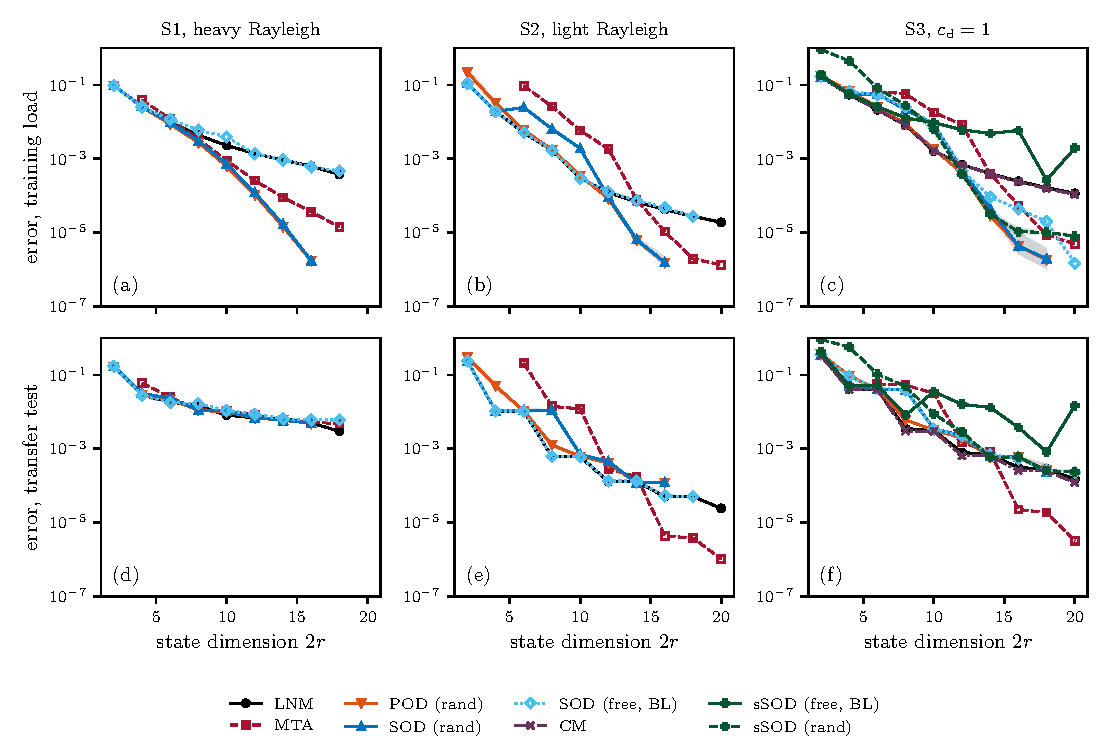
\includegraphics[width=\textwidth]{fig_c_error.pdf}
\caption{ROM displacement error against state dimension $2r$, median and interquartile range over 20 realizations. Columns: S1 with heavy Rayleigh damping; S2 with light Rayleigh damping; S3 with $c_{\mathrm d}=1$. Top: new random load at the training location. Bottom: transfer test (free decay from a floor-4 point load for S1; random mid-span load for S2 and S3). Training signal in brackets; free, BL: order-matched band-limited decay; sSOD: state-space SOD; CM: complex-mode truncation.}
\label{fig:error}
\end{figure}
So the same random-trained basis is worse than the LNMs at intermediate order and better at high order, and the gain belongs to the training load. Sections~\ref{sec:adds} and \ref{sec:displace} explain both.



\section{What the record adds}\label{sec:adds}
Is the high-order gain of a random-trained SOD basis the static correction, and does it serve only the loads the record saw?
We answer first by the geometry of the basis and then by moving the load.

\paragraph{Containment of the static vectors.} Figure~\ref{fig:static}a gives the containment residual \eqref{eq:contain} of the two static load vectors of S2, $\bK^{-1}\bm{b}_{\mathrm{tip}}$ and $\bK^{-1}\bm{b}_{\mathrm{mid}}$, with light damping and the 20 random tip records of Section~\ref{sec:acc}.
\begin{itemize}
\item At $r=8$ the SOD subspace holds the tip vector to $\rho=1.8\times10^{-7}$ (median), against $3.3\times10^{-5}$ for the LNMs, about 190 times closer. At $r=7$ the figures are $1.6\times10^{-6}$ and $5.2\times10^{-5}$.
\item It holds the mid-span vector no better than the LNMs: $7.9\times10^{-5}$ against $3.7\times10^{-5}$ at $r=8$. The record never saw that load.
\item The SOD basis of the order-matched band-limited decay contains no static correction. Its residuals equal those of the LNMs within 12\,\% ($3.6\times10^{-5}$ for the tip vector at $r=8$), as its LNM-level errors in Figure~\ref{fig:error} require.
\end{itemize}
POD of the same records contained the tip vector equally well ($1.7\times10^{-7}$ at $r=8$). At the data rank the two span one subspace.

\paragraph{Principal angles.} At $r=8$, seven of the eight principal angles between the SOD subspace and MTA with the tip vector only were below $0.03^\circ$ (medians); the eighth was $13^\circ$ (at most $15^\circ$). Against the eight LNMs, six angles were below $0.01^\circ$, then $2^\circ$ and $50^\circ$. Against MTA with both static vectors, the largest angle was $69^\circ$, because the mid-span vector is missing.
The random record thus supplies the LNMs it excites and, in place of LNM~8, the static correction of the load it saw.

\begin{figure}[tbp]
\centering
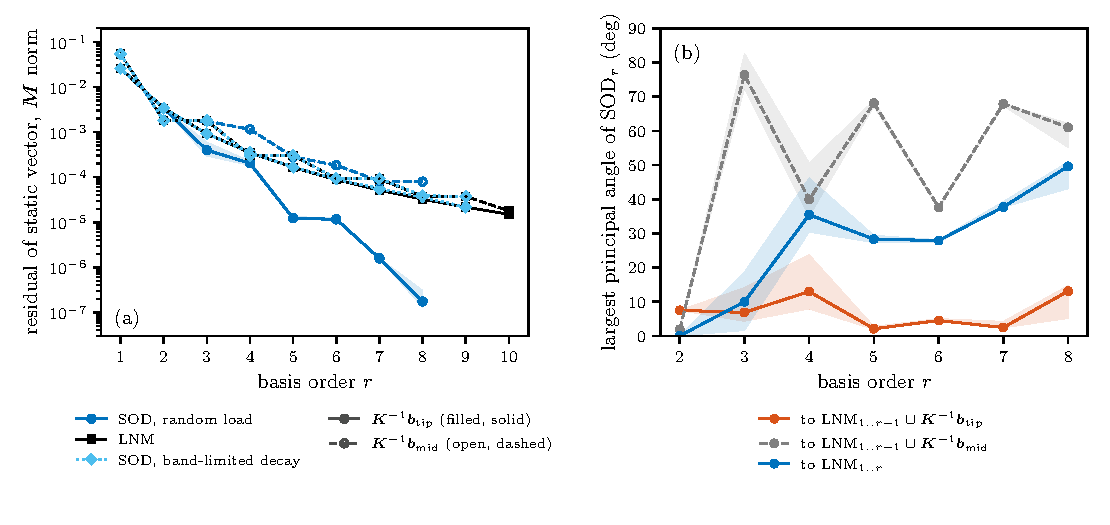
\includegraphics[width=\textwidth]{fig_c_static.pdf}
\caption{What a random tip record adds to the SOD basis; S2, light Rayleigh damping, 20 realizations. (a) Containment residual \eqref{eq:contain} of the static load vectors $\bK^{-1}\bm{b}_{\mathrm{tip}}$ (filled, solid) and $\bK^{-1}\bm{b}_{\mathrm{mid}}$ (open, dashed) against the basis order $r$: SOD of the random tip records (median and interquartile range), LNMs, and SOD of the order-matched band-limited decay. (b) Largest principal angle ($\bM$ metric) between the first $r$ SOD directions and the first $r$ LNMs, and between them and the first $r-1$ LNMs augmented by one static vector; median and range. Scripts: \texttt{g1\_static\_containment.py}, \texttt{g3\_third\_direction.py}, \texttt{mkfig\_c\_static.py}.}
\label{fig:static}
\end{figure}

\paragraph{Transfer: the gain stays at the load locations each basis was given.} For a random load at mid-span, the bases trained at the tip lost their advantage. MTA as defined above contains the static vector of the mid-span load. We therefore also built MTA with the tip vector only. We also trained data bases on independent random loads at both locations. At $r=8$ on the mid-span test:
\begin{itemize}
\item tip only: SOD erred by $1.2\times10^{-4}$ (S2, light) and $3.1\times10^{-4}$ (S2, heavy). MTA with the tip vector erred by $1.1\times10^{-4}$ and $2.9\times10^{-4}$, and the LNMs by $4.8\times10^{-5}$ and $1.4\times10^{-4}$;
\item both locations: SOD erred by $6.0\times10^{-6}$ and $9.0\times10^{-6}$; MTA by $4.2\times10^{-6}$ and $7.9\times10^{-6}$.
\end{itemize}
On S3 the pattern held. SOD and MTA from one location erred by $2.7$--$6.0\times10^{-4}$. From both locations, MTA erred by $1.0$--$2.3\times10^{-5}$ and SOD by $1.9$--$7.8\times10^{-5}$.
So on S2 and S3, SOD and MTA gained at the same load locations: those each basis was given. SOD needs response records at those locations.
On S2 at $r=7$, SOD and LNM were within 10\,\% of each other. The LNM curve for the mid-span load is a staircase, flat at $r=3$, 5 and 7. Mid-span lies within 2\,\% of a node of modes 3, 5 and 7.
On S1 the transfer test, a free decay from a point load at floor 4, was nearly basis-independent. All bases stayed within a factor of 2.1 of one another for $r=3$--9. None was consistently best.
MTA is not uniformly better. On the S2 free-decay test it was 44 times worse than the LNMs at $r=3$. At $r=8$ it was about twice as poor. On S1 it did not beat the LNMs on the floor-4 decay.
The data-driven gain is the persistence problem of \citet{Ilbeigi2017}, seen in a linear system: on S2 and S3 the data bases gained only at the load locations of their records.

\paragraph{Noisy training records.} The gain above used model kinematics. With white noise of 60 or 40\,dB on all 60 training displacements, smoothed before differentiation, the S2 error stopped falling at $r=6$--7. At $r=8$ on the training load SOD erred by $1.4\times10^{-4}$ (light damping, 60\,dB) and $1.4\times10^{-2}$ (40\,dB), against $1.5\times10^{-6}$ with model kinematics; at 40\,dB it was 11--300 times worse than the LNMs (Section~\ref{sec:s-noise}). The high-order gain therefore needs clean training records. For model reduction they come from the model.



\section{Why low orders fail}\label{sec:displace}
Why is the random-trained basis worse than the LNMs at $r=3$--5, when it holds the useful direction?
Figure~\ref{fig:static}b and the LNM content of each SOD subspace answer it.

\paragraph{One direction, ranked too early.} The SOD subspace of order $r$ held only $r-1$ LNMs for $r=3$--7 (median $\bM$-residual of each LNM below 0.1). At $r=3$ it held modes 1 and 2; LNM~3 had residual 0.17. At $r=5$ it held modes 1--4, and at $r=6$ modes 1--5, all the modes inside the load band.
The extra direction is the tip static correction. From $r=3$ on, the SOD subspace lay within $2$--$13^\circ$ (medians) of the first $r-1$ LNMs augmented by $\bK^{-1}\bm{b}_{\mathrm{tip}}$. It lay $10$--$50^\circ$ from the first $r$ LNMs, and $38$--$76^\circ$ from the first $r-1$ LNMs augmented by the mid-span vector (Figure~\ref{fig:static}b).
The direction enters at $r=3$ because it is smoother than the upper in-band modes: the third SOD frequency of a random record was 47.7, between modes 2 and 3 (Section~\ref{sec:mix}).
The errors follow the count of in-band modes. Against the LNM ROM the SOD ROM was 4.8 times worse at $r=3$ and 6.5 times worse at $r=5$, while it lacked one in-band mode. At $r=6$, with all five in-band modes present, it was 1.4 times better. At $r=7$ and 8 it was 11 and 27 times better.
The direction that carries the gain at high order is the one that causes the loss at low order.

\subsection{Mixing by training signal}\label{sec:mix}
The same ranking explains how the training signal shapes the basis.
Figure~\ref{fig:mac} compares configuration SOD modes with LNMs by the mass-weighted modal assurance criterion (MAC; \citealp{Allemang2003}; one realization).
\begin{itemize}
\item \emph{Free decay, proportional damping.} On S2, SOD modes 1--8 matched LNMs 1--8 with MAC $\ge0.93$. Frequencies of modes 1--6 were within 0.03--1.6\,\%. The modal coordinates were nearly uncorrelated (largest correlation 0.07).
\item \emph{Random and swept sine.} Extra smooth directions appeared between genuine modes. On S2 with random data, SOD returned frequencies 3.5, 22.0, 47.7, 62.2, 121, 200. The third is a mixture of LNMs 1--3 (MAC 0.19, 0.28, 0.51): the quasi-static tip direction of Section~\ref{sec:displace}. The sweep inserted a direction at 17.1, below mode 2.
\item \emph{Free decay with the dashpot.} Non-proportional damping correlates the modal coordinates (0.71). Configuration SOD modes 2--4 mixed (MAC 0.82, 0.86, 0.58), as the exactness criterion predicts.
\end{itemize}
Every direction ranked among the modes shifts the genuine modes down one rank. A truncated basis then omits a mode it needs, which explains the intermediate-order errors.
State-space SOD on S3 behaves in the same way, plane by plane (Section~\ref{sec:s-smix}).

\begin{figure}[tbp]
\centering
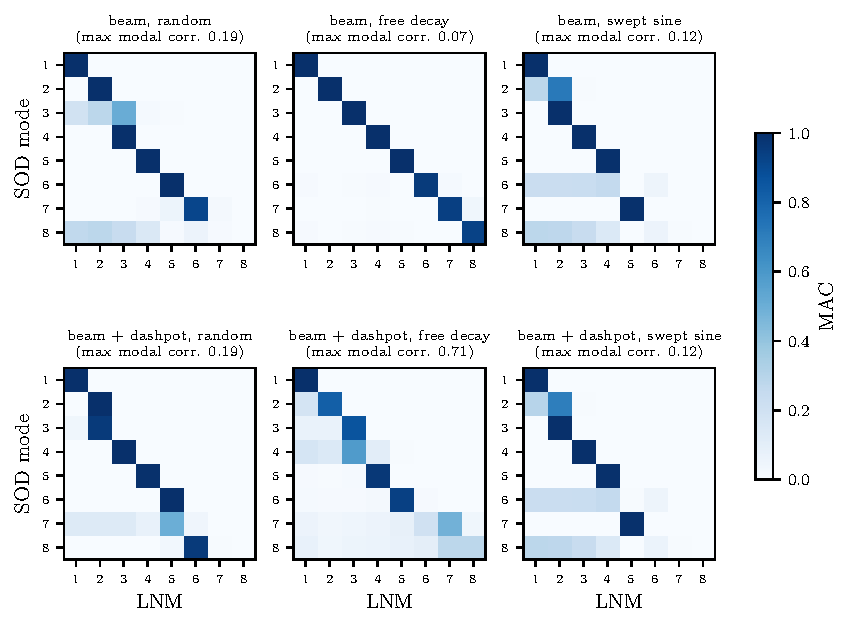
\includegraphics[width=0.92\textwidth]{fig_c_mac.pdf}
\caption{MAC between configuration SOD modes 1--8 (rows, smoothest first) and LNMs 1--8 (columns); the training data excite no higher modes. Top: S2, light damping. Bottom: S3, $c_{\mathrm d}=0.2$. Columns: training signal.}
\label{fig:mac}
\end{figure}

Smaller rank tolerances admit a second kind of smooth non-modal direction: weakly excited ones, whose mean-square frequency is set by how little they move, not by a mode (Section~\ref{sec:rank}).
A free decay under proportional damping avoids the displacement, because it contains no quasi-static response. A forced record contains it, and ranking by smoothness misplaces it.


\section{Removing the loss: recognising modes}\label{sec:noise}
How can the quasi-static direction be kept without letting it displace a mode?
For model reduction the kinematics come from the model: velocities and state derivatives are exact, and no measurement noise enters.
Modes are therefore recognised, paired and ordered by their own frequency or circularity, never by their SOD value. Smoothness says how slowly a projection moves. It does not say which mode the projection belongs to, as Sections~\ref{sec:displace} and \ref{sec:rank} show.

\subsection{Recognising modes}\label{sec:recog}
\paragraph{Configuration SOD: spectral consistency.} A coordinate that is a single real mode has its mean-square frequency at its spectral peak. A mixture of modes does not. We read each coordinate's spectrum from its periodogram of the type-II discrete cosine transform (DCT-II), smoothed over $\pm2\,\%$ in frequency. A raw periodogram of a randomly forced coordinate has single-bin spikes. Its arg-max is then not the resonance, and its bin-level width misses the damping width $2\zeta\omega$. Coordinate $i$ is kept if its peak lies within $\max(5\,\%,\,w_i)$ of its SOD frequency $\sqrt{\mu_i}$. Here $w_i$ is the relative half-power width of that peak, capped at 15\,\%. The width makes the test damping-aware. The cap matters. A drifting or broadband coordinate peaks near zero frequency, with a width above 1, and would otherwise pass. The test assumes one frequency per coordinate. A nonlinear decay sweeps that frequency, and the test can then reject a genuine NNM (Section~\ref{sec:nlbb}). Circularity needs no fixed frequency. Two kept coordinates that share one peak cannot both be that mode. The one carrying more response energy, $\|\bphi_i\|^2\avg{q_i^2}$, is kept. Recognised modes are ordered by peak frequency.
Applied with a fixed 5\,\% tolerance to the ten smoothest coordinates of clean S2 records, the test rejected 108 of 134 spurious directions and no genuine mode (10 realizations, tolerances $10^{-10}$--$10^{-14}$; Section~\ref{sec:s-recog} compares two other rules).

\paragraph{State SOD: circularity.} Consider the two coordinates of a modal plane. Up to a real change of basis, they are the real and imaginary parts of one complex modal coordinate. SOD returns them uncorrelated and with unit variance, so in their own plane the cloud is round. Read as $z=q_a+\mathrm i\,q_b$, the pair rotates one way and the spectrum of $z$ is one-sided. Two unrelated coordinates, or coordinates of two different planes, give a nearly symmetric spectrum.
Pairs are therefore formed by matching, not by rank. Candidate pairs are paired greedily by one-sidedness and kept above 0.85; only one plane is kept per frequency. A loose frequency gate, four times the spectral tolerance, only limits the search. The plane frequency is the peak of the one-sided spectrum of $z$, and planes are ordered by it.
Pairing by rank fails: pairing adjacent coordinates in SOD order lost the slowest plane of random-load records, because a quasi-static coordinate sat between its two members. With smoothed spectra and the loose gate, the mode-1 plane was recognised in all 8 test records. Modal planes gave a one-sidedness of 0.89--0.99, other pairs 0.51--0.75. Section~\ref{sec:s-recog} gives the rule for a plane contaminated by another mode at its own frequency.

\subsection{Selection for model reduction}\label{sec:romsel}
We compared two bases from the same SOD, with model kinematics (10 realizations):
\begin{itemize}
\item R0: the plain basis, in SOD order;
\item RHB: the recognised modes or planes inside the load band, $\omega\le\omega_{\mathrm c}$, first, ordered by frequency; then the remaining coordinates in SOD order.
\end{itemize}
Section~\ref{sec:s-recog} compares four other orders.
Modes above the load band respond quasi-statically to it. The smooth direction that carries that response serves a ROM better than the mode itself. This is why RHB stops at $\omega_{\mathrm c}$.
\paragraph{S2, random tip load.} RHB removed the low-order damage of spurious directions. In no record was it more than 11\,\% worse than R0 at any order.
\begin{itemize}
\item Tolerance $10^{-12}$: the median two-mode error fell from $1.1\times10^{-1}$ to $2.0\times10^{-2}$ on the training load. At mid-span it fell from $2.2\times10^{-1}$ to $1.0\times10^{-2}$. The four-mode errors fell from $6.1\times10^{-3}$ to $1.8\times10^{-3}$ and from $1.0\times10^{-2}$ to $6.5\times10^{-4}$.
\item Tolerance $10^{-10}$: the four-mode mid-span error fell from $1.1\times10^{-2}$ to $7.6\times10^{-4}$.
\item At $r=6$ RHB equalled R0 at tolerance $10^{-10}$ and improved it at $10^{-12}$ ($1.7\times10^{-4}$ to $1.0\times10^{-4}$ on the training load). At $r=8$ all bases erred by $1.4\times10^{-6}$ on the training load.
\end{itemize}
\paragraph{S3, $c_{\mathrm d}=0.2$, state SOD.} From random-load records RHB improved state dimension 4 in every record (median training-load error $2.9\times10^{-1}\to1.0\times10^{-1}$, mid-span $3.7\times10^{-1}\to9.2\times10^{-2}$). At state dimension 8 it was slightly worse (median ratio 1.1--1.2, at most 2.5 in one record). From 12 on it equalled R0. Planes from forced records are tilted by their quasi-static response (Section~\ref{sec:ic}). From the band-limited decay the recognised order matched the SOD order, and all bases were identical.
For model reduction we therefore recommend RHB. Recognised in-band modes come first, by frequency; the rest follow in SOD order.
Recognition thus keeps the static-correction direction in the basis but places it behind the in-band modes it displaced.


\section{How far the explanation reaches}\label{sec:reach}
Does the explanation hold where the modes are complex, and where the structure is nonlinear? We test state-space SOD on S3, and two nonlinear cantilevers: S4 for backbone accuracy and S5 for forced bifurcations.

\subsection{Complex modes}\label{sec:complex}
On S3 the modes are complex, and configuration SOD from a free decay mixed modes 2--4 (MAC 0.82, 0.86 and 0.58; Section~\ref{sec:mix}). Complex modes themselves bought little on the forced tests: a configuration ROM on the undamped LNMs, with the full damping matrix projected, erred within 25\,\% of complex-mode truncation at every order. Configuration SOD fails on S3 because its modes mix, not because the true modes are complex.
State-space SOD of the order-matched band-limited decay mixed them much less. On the forced tests at state dimension 8 it came within a factor of 2.7 of complex-mode truncation, and it cut the mid-span error of configuration SOD by 5--13 times. Above state dimension 8 its error stalled near $10^{-3}$ on the random test: weakly excited planes are poorly determined by a decay. No energy-Galerkin state ROM was unstable.
The planes follow the record, as the configuration modes did. A decay tilts them toward the modes it excites above the retained band; where the leakage exceeded 0.05, the ROM converted it into a relative eigenvalue error of 0.2--0.8 times its square. Of the decays tested, those with little energy above the retained band, relative to the energy inside it, gave the most accurate state ROMs: static release, and band-limited decays matched to the ROM order. A forced record tilts the planes by its quasi-static response; state SOD from random records erred by $6.1\times10^{-1}$ at state dimension 2 ($c_{\mathrm d}=0.2$). Section~\ref{sec:s-complex} gives the errors per case, the trajectories and the training-decay study.

\subsection{A nonlinear backbone}\label{sec:nlbb}
Nonlinear ROMs proper reduce onto invariant manifolds: nonlinear normal modes \citep{Shaw1993,Touze2004} and spectral submanifolds \citep{Haller2016,Cenedese2022}. Model-based alternatives augment the modes with static or derivative vectors, or with a quadratic manifold built from them \citep{Idelsohn1985,Jain2017}; \citet{Mignolet2013} review non-intrusive ROMs of geometrically nonlinear structures, including the choice of basis; \citet{Touze2021} review invariant-manifold methods and the quadratic manifold. We do not compete with them. We test linear Galerkin bases only, where SOD is an alternative to LNM, MTA and POD. Here the question is narrower: does the static-correction explanation account for what a decay-trained basis gains on a structure with a local nonlinearity?
S4 is the COST F3 cantilever of Section~\ref{sec:bench} (Figure~\ref{fig:systems}d).

\paragraph{Reference backbone.} We computed the NNM1 backbone \citep{Kerschen2009} of the full model by odd harmonic balance \citep{Detroux2015}. It used eight harmonics and pseudo-arclength continuation.
We integrated the full model over one period from the balanced initial state, at four energies. It returned to that state within $1.5\times10^{-10}$ or better.
The backbone rises from 23.66\,Hz to 42.1\,Hz at total energy $H=3\times10^{-2}$\,J.
A 5:1 internal resonance with mode 2 (148.3\,Hz) forms a tongue at 29.9--30.4\,Hz (Figure~\ref{fig:nl}a). The main backbone is interrupted between $H=3.6\times10^{-3}$ and $4.0\times10^{-3}$\,J, where the tongue branches off. The tongue itself stays near 30\,Hz up to the highest energy computed.
There the fifth harmonic exceeds the fundamental. We compare backbones outside the tongue only.
Plucked responses from static deflections are not on the backbone. Their zero-crossing frequencies lay up to 3\,\% below it at the same energy. The plucked state also excites higher modes.

\paragraph{Bases.} LNM; MTA with the static tip-load vector; and SOD and POD of one damped decay ($\zeta=0.01$, Rayleigh on modes 1--2). Two decays were used. The band-limited decay follows the convention of Section~\ref{sec:bench}. It is an equal-energy sum of LNMs 1--4, the band of interest for $r\le4$. The static-release decay starts from the deflection under a 30\,N tip load. The results below are for static release; the band-limited decay follows them. It lasts 1.5\,s and sweeps the energy down the backbone.
Each ROM backbone was computed by the same harmonic balance on the reduced equations.

\paragraph{Results.} Median backbone frequency errors over 24 energies outside the tongue, from $6\times10^{-4}$ to $2.5\times10^{-2}$\,J (Figure~\ref{fig:nl}b):
\begin{itemize}
\item $r=1$: LNM $1.1\times10^{-2}$, SOD and POD $2.2\times10^{-3}$;
\item $r=2$: LNM $1.5\times10^{-3}$, MTA $8\times10^{-5}$, SOD $1.4\times10^{-4}$, POD $2.1\times10^{-4}$;
\item $r=3$: LNM $4.7\times10^{-4}$, MTA $1.4\times10^{-6}$, SOD $2.0\times10^{-6}$, POD $1.2\times10^{-5}$;
\item $r=4$: LNM $2.0\times10^{-4}$, MTA $1.4\times10^{-6}$, SOD $5\times10^{-7}$, POD $4\times10^{-7}$.
\end{itemize}
At $r=3$ and 4, decay-trained bases improved the backbone by two to three decades over the LNMs. At $r=2$ the gain was about one decade. The model-based static tip-load vector did as well or better at $r=2$ and 3, and SOD was better at $r=4$.
Both contain the deformation that the localized cubic force imposes on the beam: MTA as $\bK^{-1}\bm{e}_{\mathrm{tip}}$, SOD in its first direction, which lies $3\times10^{-4}$ degrees from $(\bK-\omega^2\bM)^{-1}\bm{e}_{\mathrm{tip}}$ at the first SOD frequency of the 30\,N decay, $\omega=196.0$\,rad/s (\texttt{n14\_bent\_mta.py}).
SOD led POD at $r=2$ and 3; at $r=4$ POD was 1.4 times better.

\paragraph{Held-out time-domain tests.} Conservative responses started from static deflections not used in training. The loads were 3, 10 and 20\,N at the tip and 20 and 60\,N at mid-span.
At $r=4$, MTA, SOD and POD gave displacement errors of $1.5$--$5.5\times10^{-3}$ over 0.1\,s. The LNMs gave $4.5\times10^{-4}$ to $1.1\times10^{-2}$, better at low energy and worse at high energy. Zero-crossing frequency errors were at most $1.1\times10^{-4}$ for SOD and MTA, and up to $9.1\times10^{-4}$ for the LNMs.
At $r=2$, SOD gave displacement errors of $0.8$--$4.8\times10^{-2}$, MTA $4$--$13\times10^{-2}$.
The plucked states excite modes that a backbone-dominated record does not contain. At $r=4$ displacement accuracy in these tests was therefore limited by the truncated modes: MTA, SOD and POD gave errors within the same range.
The four-mode SOD ROM matched the backbone to about $10^{-6}$ up to 0.048\,J, about three times the $1.48\times10^{-2}$\,J of its training state; there an internal-resonance tongue of the ROM itself begins (Figure~\ref{fig:track}). Section~\ref{sec:s-s4} gives the band-limited training decay, the backbone read from the record alone, the out-of-plane bend of the NNM and the integration cost.

\paragraph{The bent correction as a basis vector.} With $(\bK-\omega^2\bM)^{-1}\bm{e}_{\mathrm{tip}}$ at $\omega=196.0$\,rad/s in place of the static vector, the one-mode ROM equalled the one-mode SOD ROM ($2.2\times10^{-3}$). At $r=2$ it was the most accurate basis: backbone error $4.7\times10^{-5}$, against $8.0\times10^{-5}$ for MTA and $1.4\times10^{-4}$ for SOD. At $r=3$ and 4 it equalled MTA, $1.4\times10^{-6}$, while SOD reached $5.2\times10^{-7}$ at $r=4$. The four-mode SOD subspace differs from that of MTA in one direction, by $1.75^\circ$. No model-built set we formed reproduced that direction (Section~\ref{sec:s-s4}).

\begin{figure}[tbp]
\centering
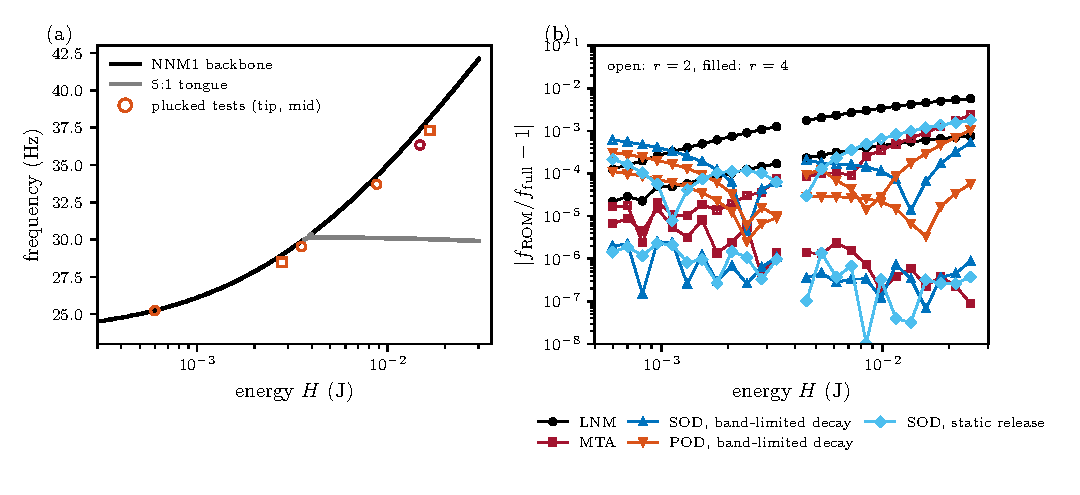
\includegraphics[width=\textwidth]{fig_c_nl.pdf}
\caption{COST F3 cantilever with cubic tip spring. (a) Frequency--energy plot of NNM1 from harmonic balance: main backbone, 5:1 tongue, and zero-crossing frequencies of the plucked tests. Circles: tip loads; squares: mid-span loads; dark: the 30\,N training state. (b) Backbone frequency error of the ROMs against energy, outside the tongue; open: $r=2$, filled: $r=4$. SOD and POD from the band-limited decay (LNMs 1--4, equal energy), and SOD from the static release.}
\label{fig:nl}
\end{figure}

\subsection{Bifurcation diagrams of a two-well beam}\label{sec:moon}
A backbone tests free motion on one NNM. Forced motion between two potential wells is harder. It has coexisting attractors, period doubling and chaos. S5 is a cantilever of this kind, after the magneto-elastic beam of \citet{Moon1979}.

\paragraph{Model.} Ten Hermite elements, $EI=m'=L=1$ as for S2, $n=20$. A tip force $f=-k_1x+k_3x^3$, with $x$ the tip deflection, $k_1=6$ and $k_3=300$, stands in for the magnets. Since $k_1$ exceeds the tip stiffness $3EI/L^3$, the straight state is unstable. Two buckled equilibria have tip deflection $\pm x^*=\pm0.1$. Linearized there, the first three frequencies are $\omega_{\mathrm w}=4.90$, 22.3 and 61.8; the clamped beam has 3.52, 22.0 and 61.7. Rayleigh damping gives $\zeta=0.02$ at the first two well modes. The base acceleration is $A\cos\varOmega t$. All models were integrated by average-acceleration Newmark \citep{Newmark1959} with Newton iterations, at 100 steps per forcing period.

\paragraph{Training and bases.} One cross-well free decay trained the data bases. It started at $+x^*$ with the velocity of a unit step in base velocity. Over 60 time units the tip swept $\pm2.5x^*$ and crossed zero 18 times, the last at $t=14.1$. It then settled in a well. Velocities came from the model.
\begin{itemize}
\item POD and SOD used second moments about zero, so the buckled equilibria stay in the span. The data rank was 11.
\item The first POD direction held 98.7\,\% of the variance. The SOD frequencies were 2.49, 10.4, 23.8 and 60.8. The second SOD direction is not modal: its MAC with the second well LNM was 0.05.
\item MTA used $r-1$ clamped LNMs plus $\bK^{-1}\bm{e}_{\mathrm{tip}}$, the static vector of the nonlinear force. Two LNM bases were also tested: clamped, and linearized in a well.
\end{itemize}
The first SOD direction lies $0.7^\circ$ from $\bK^{-1}\bm{e}_{\mathrm{tip}}$ in the mass metric.

\paragraph{Diagrams.} The forcing parameter was swept up and down. The state was carried from one value to the next. After a transient, the tip displacement was sampled once per period at phase $\varOmega t=0 \bmod 2\uppi$. A response is called periodic of period $k$ if it has $k$ distinct samples to $10^{-3}x^*$. It is cross-well if its orbit changes sign. ROM and full-model sample sets were compared by their Wasserstein distance $W_1$, divided by $x^*$. In-well orbits were also compared by their extremes. A ROM may settle on the mirror orbit, $-x(t+\uppi/\varOmega)$, in the other well. That is a choice between coexisting attractors, not a model error, so the mirror orbit is compared instead.

\paragraph{Amplitude sweep.} At $\varOmega=0.85\,\omega_{\mathrm w}$, $A$ ran from 0.01 to 0.30 in steps of $10^{-3}$, with 150 transient and 64 sampled periods (Figure~\ref{fig:mbamp}). The cascade was resolved in steps of $10^{-4}$ with 300 transient periods (Figure~\ref{fig:mbcasc}). On the up sweep the full model showed:
\begin{itemize}
\item a small in-well orbit, which jumped to a resonant in-well orbit at $A=0.075$;
\item period doubling at $A=0.1286$ (period 2), 0.1396 (period 4) and 0.1410 (period 8);
\item escape to cross-well chaos at 0.1412, a period-5 window at 0.173--0.181, and cross-well period-1 motion above 0.238.
\end{itemize}
Period 16 lay within one step of $10^{-4}$. On the down sweep, cross-well period-1 motion persisted to $A=0.093$.

\paragraph{One mode.} One-mode ROMs reproduced the sequence but shifted it in amplitude. The onset of period 2 moved by $-1.5\,\%$ (SOD), $-1.3\,\%$ (POD) and $-5.6\,\%$ (MTA). It moved by $+4.4\,\%$ (clamped LNM) and $+18\,\%$ (LNM in the well). The escape moved by about as much. The shift follows the one-mode model itself. With $\bphi$ scaled to unit tip displacement, it reads $\bar m\ddot q+\bar c\dot q+(\bar k-k_1)q+k_3q^3=-\varGamma\bar m\,a_{\mathrm g}$. Here $\bar m$, $\bar c$ and $\bar k$ are the modal mass, damping and stiffness, $\varGamma$ is the participation factor and $a_{\mathrm g}$ the base acceleration. Its equilibrium is $q^*=\sqrt{(k_1-\bar k)/k_3}$ and its well frequency $\sqrt{2(k_1-\bar k)/\bar m}$ (Table~\ref{tab:moon}). The static vector gives the exact equilibrium but a light modal mass, so its well frequency is 3.0\,\% high. The LNM in the well is 9.3\,\% low. SOD balances the two errors. A high well frequency moved the cascade to lower amplitude, and a low one to higher amplitude.


\paragraph{Which vector is the first SOD direction?} The magnets act as a rank-one stiffness at the tip. The deflection under a harmonic tip force at frequency $\omega$, $\bm{d}(\omega)=(\bK-\omega^2\bM)^{-1}\bm{e}_{\mathrm{tip}}$, therefore runs from the static vector at $\omega=0$ to the in-well LNM at $\omega=\omega_{\mathrm w}$: the in-well mode satisfies $(\bK-\omega_{\mathrm w}^2\bM)\bphi=-\kappa\phi_{\mathrm{tip}}\bm{e}_{\mathrm{tip}}$, with $\kappa$ the linearized magnet stiffness. The first SOD direction lies on this curve. It is $0.69^\circ$ from $\bm{d}(0)$, $2.2^\circ$ from $\bm{d}(\omega_{\mathrm w})$, and $0.003^\circ$ from $\bm{d}(2.42)$; at the first SOD frequency, 2.49, the angle is $0.05^\circ$ (\texttt{mb10\_dynamic\_correction.py}). With $\bm{d}(2.42)$ as its one vector, a one-mode ROM reproduced SOD: equilibrium $-0.32\,\%$ and well frequency $+1.26\,\%$, against $-0.32\,\%$ and $+1.25\,\%$. On the amplitude sweep its in-well extreme error was $1.38\times10^{-2}$, against $1.37\times10^{-2}$ for SOD and $2.56\times10^{-2}$ for MTA, and its cascade landmarks matched those of SOD at the sweep step of $10^{-3}$. The one-mode advantage of SOD over MTA is therefore the static correction bent by inertia at the frequency of the training record.

\paragraph{More modes.} At $r=2$ SOD, POD and MTA placed the period-2, period-4 and escape amplitudes within one step of $10^{-4}$; the two LNM bases still erred by 0.6--3\,\%. Which of SOD and MTA is closer at $r=2$ depends on the measure: SOD erred less on the in-well orbit extremes ($1.5\times10^{-4}$ against $3.3\times10^{-4}$), MTA on the in-well Wasserstein distance ($2.0\times10^{-5}$ against $7.9\times10^{-5}$; Table~\ref{tab:s-moon}). Replacing the static vector of MTA by $\bm{d}(2.42)$ did not move it toward SOD on the extremes ($3.1\times10^{-4}$). From $r=3$ MTA was the most accurate basis and SOD second (Table~\ref{tab:moon}). Classification agreed with the full model at 98.5--99.5\,\% of the 582 points for SOD, MTA and POD at $r\ge2$. The remaining points lie at the edges of the chaotic windows.

\paragraph{Frequency sweep.} At $A=0.3$, $\varOmega$ ran from 0.2 to 1.4 $\omega_{\mathrm w}$ (Section~\ref{sec:s-s5}). At $r\ge2$ every ROM placed the jumps into and out of cross-well motion within $0.04\,\omega_{\mathrm w}$, and from $r=3$ the ranking of the amplitude sweep returned (Table~\ref{tab:moon}).

\begin{table}[tbp]
\centering\small
\caption{Two-well beam (S5). One-mode ROMs: relative errors of the equilibrium $q^*$ and the well frequency. Then the median error of the response against $r$. Amplitude sweep: in-well orbit extremes, divided by $x^*$. Frequency sweep: $W_1/x^*$ on the periodic points.}
\label{tab:moon}
\setlength{\tabcolsep}{3pt}
\resizebox{\textwidth}{!}{\begin{tabular}{lrrcccccccc}
\toprule
 & \multicolumn{2}{c}{one mode} & \multicolumn{4}{c}{amplitude sweep, $r=1$--4} & \multicolumn{4}{c}{frequency sweep, $r=1$--4}\\
\cmidrule(lr){2-3}\cmidrule(lr){4-7}\cmidrule(lr){8-11}
basis & $q^*$ & $\omega_{\mathrm w}$ & 1 & 2 & 3 & 4 & 1 & 2 & 3 & 4\\ \midrule
SOD & $-0.3\,\%$ & $+1.3\,\%$ & $1.4\times10^{-2}$ & $1.5\times10^{-4}$ & $8.5\times10^{-7}$ & $3.3\times10^{-8}$ & $2.0\times10^{-2}$ & $1.4\times10^{-3}$ & $1.8\times10^{-6}$ & $1.8\times10^{-7}$\\
POD & $-0.3\,\%$ & $+1.2\,\%$ & $1.4\times10^{-2}$ & $1.5\times10^{-4}$ & $1.1\times10^{-5}$ & $3.8\times10^{-7}$ & $2.2\times10^{-2}$ & $1.0\times10^{-3}$ & $3.5\times10^{-5}$ & $2.8\times10^{-6}$\\
MTA & $0$ & $+3.0\,\%$ & $2.6\times10^{-2}$ & $3.3\times10^{-4}$ & $2.4\times10^{-7}$ & $4.8\times10^{-9}$ & $1.8\times10^{-2}$ & $2.2\times10^{-3}$ & $2.1\times10^{-6}$ & $9.6\times10^{-8}$\\
LNM, clamped & $-1.5\,\%$ & $-1.5\,\%$ & $2.0\times10^{-2}$ & $3.1\times10^{-3}$ & $9.6\times10^{-4}$ & $4.1\times10^{-4}$ & $2.2\times10^{-2}$ & $2.2\times10^{-3}$ & $7.5\times10^{-4}$ & $3.0\times10^{-4}$\\
LNM, in well & $-6.5\,\%$ & $-9.3\,\%$ & $1.2\times10^{-1}$ & $1.5\times10^{-2}$ & $4.5\times10^{-3}$ & $1.9\times10^{-3}$ & $3.1\times10^{-2}$ & $5.5\times10^{-3}$ & $1.4\times10^{-3}$ & $6.1\times10^{-4}$\\
\bottomrule
\end{tabular}}
\end{table}

\begin{figure}[tbp]
\centering
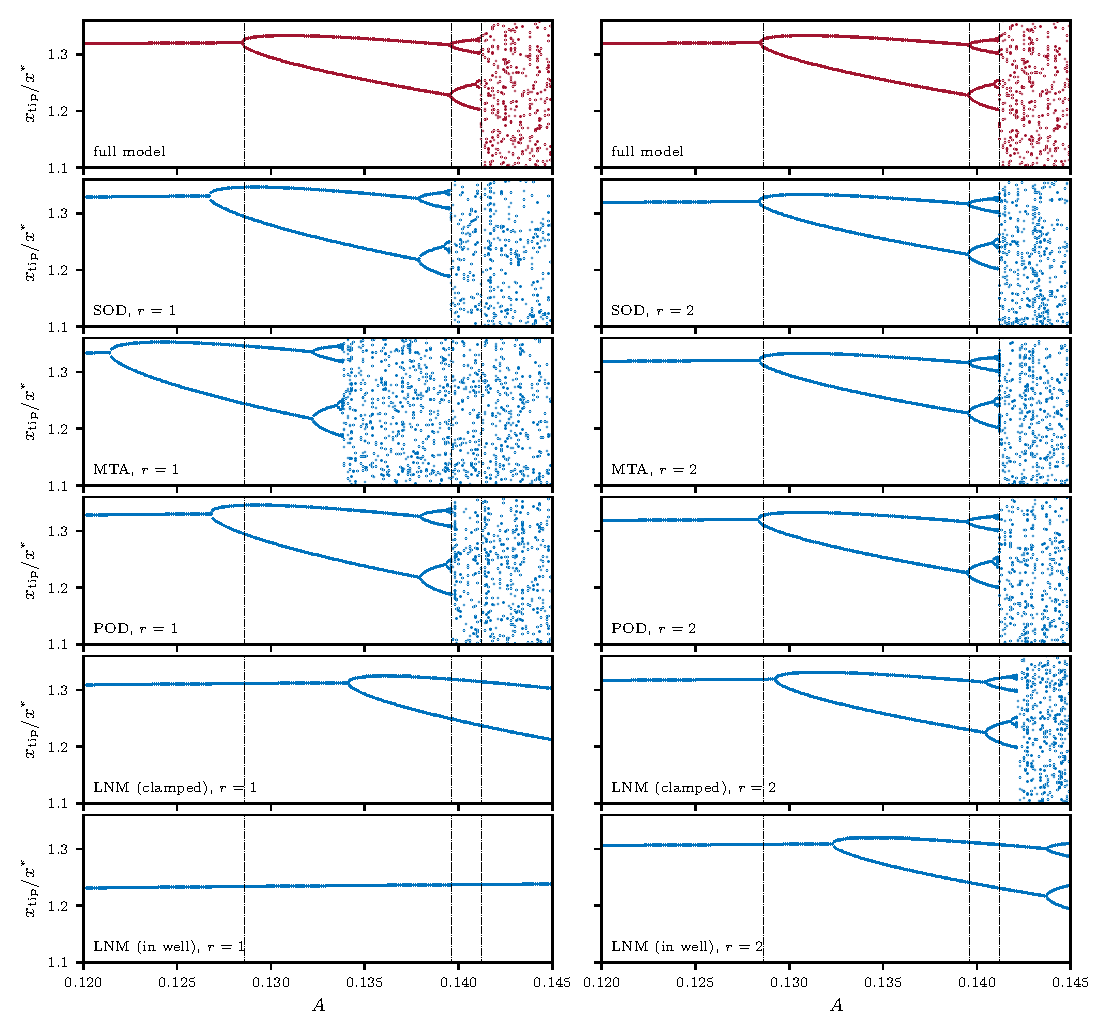
\includegraphics[width=\textwidth]{fig_mb_cascade.pdf}
\caption{The period-doubling cascade of Figure~\ref{fig:mbamp}, up sweep in steps of $10^{-4}$. ROMs on the mirror orbit are shown through it. Dotted: full-model onsets of period 2 and period 4, and the escape to cross-well motion. Left $r=1$, right $r=2$. The cascade of the in-well LNM ROM at $r=1$ lies above $A=0.15$.}
\label{fig:mbcasc}
\end{figure}

\paragraph{What the two-well beam adds.} It shows where model-based correction accounts for the data advantage. One cross-well decay gave SOD the correction at the nonlinear force without its location. At one mode that correction is bent by inertia at the record's frequency, and it beats the static vector; the same bent vector, built from the model, does as well. At $r=2$ SOD and MTA trade places by measure. From $r=3$ the model-based MTA basis was the most accurate, and SOD followed within a factor of 7 (amplitude sweep) and 2 (frequency sweep). POD fell behind both.

\section{Computation cost}\label{sec:cost}
Are SOD ROMs faster, as reported \citep{Ilbeigi2018}, and if so, is the gain a property of SOD?
Two facts frame the answer.
A full-rank change of coordinates is a congruence of $(\bM,\bK)$ and a similarity of the first-order state matrix $\bm{A}$, so it leaves every eigenvalue unchanged.
An explicit integrator is limited by the spectral radius $\rho(\bm{A})$, not only by the highest natural frequency $\omega_{\max}$. With $\bC=\alpha\bM+\beta\bK$ the high finite-element modes are overdamped, and their real eigenvalues, about $\beta\omega^2$, can exceed $\omega_{\max}$. A change of coordinates leaves $\rho(\bm{A})$ unchanged; truncation can lower it.
What a change of coordinates can alter is how an adaptive integrator weighs its error estimate and, for an implicit integrator, how well its Newton iterations are conditioned.
We compared cost at matched integration accuracy. Each model, with each adaptive integrator (RK45 and Radau), was charged its cheapest run whose displacement error against a tight reference of the same model was at most $10^{-6}$ (protocol and table in Section~\ref{sec:s-cost}). This prices integration alone. It does not compare cost against the ROM's total error relative to the full model, which truncation sets; that comparison was not made.
On S2 under a chirp load, truncation set the cost. The full model is limited by an overdamped finite-element mode with eigenvalue $-9.3\times10^5$. RK45 needed $3.5\times10^7$ evaluations for it and $4.0\times10^4$ for the four-mode LNM ROM, about 870 times fewer.
The coordinates of a subspace did not set it. The order-8 SOD subspace needed 72\,386 RK45 evaluations in Ritz coordinates and 71\,378 in raw smooth modes; on S1 the raw basis needed 1.2 times as many. For the implicit Radau method the raw smooth modes, whose reduced mass matrix has condition number $7.4\times10^6$, needed 1.9 times the evaluations of Ritz coordinates.
At one fixed tolerance, by contrast, the same subspace needed 416\,k RK45 evaluations in raw smooth modes and 158\,k in Ritz coordinates, at errors of $2.1\times10^{-10}$ and $3.8\times10^{-9}$. An absolute tolerance weighs coordinates by their scale, and a change of coordinates changes the scale. \citet{Ilbeigi2018} reported a full-order SOD model of a nonlinear control system about twice as fast as the original; that is the size of difference coordinate scaling alone produced here at a fixed tolerance. We have not tested their system.
For SOD ROMs we recommend Ritz coordinates of the retained subspace: they decouple the reduced model and, in every case tested, were no costlier than any other basis of the same subspace.


\section{Discussion}\label{sec:disc}
The paper set out to test whether an SOD basis holds the directions its training record visits, and whether that explains its being better and worse than the LNMs at once.
The evidence supports the hypothesis on the linear benchmarks. Three findings point the same way.
First, the geometry: at high order the random-trained SOD subspace contains the static vector of the training load about 190 times better than the LNMs, and that of the unseen load no better. Seven of its eight directions coincide with MTA built on the training load alone.
Second, the transfer test: given the same load locations, SOD and MTA ROMs agreed within a factor of 3.4; with one location missing, both lost their gain.
Third, the ladder: the same quasi-static direction enters at $r=3$, displaces an in-band mode until all in-band modes are present, and the error ratio to the LNMs turns from a loss into a gain at that order: 6.5 times worse at $r=5$, 1.4 times better at $r=6$, where all five in-band modes are present. Recognising modes by frequency removed the loss.
A band-limited free decay, which contains no quasi-static response, gave a basis with no static correction and LNM-level errors, as the hypothesis requires.

SOD therefore delivers static correction from response records: at the same load locations its ROMs came within a factor of 3.4 of MTA. It needs no eigensolution of the model, but the Galerkin ROM still needs $\bM$, $\bC$ and $\bK$, and SOD needs response records at every load location of interest. These cost more to simulate than the static solves of MTA.
The static vector depends only on where a load acts: a load $\bm{b}\,g(t)$ has the static vector $\bK^{-1}\bm{b}$ for any $g$. Whether a record delivers it depends on the record. The record must contain quasi-static response of the truncated modes, so its load spectrum must lie below them; a band-limited free decay contains none. That response must survive the data rank and the noise: at 40\,dB the training noise set an error floor 11--300 times above the LNMs. And the basis order must reach the direction, which SOD ranks among the in-band modes. Within these conditions the gain carried over to new random loads at the training input; the tested histories were band-limited random loads of one bandwidth per system. Loads at several points must vary independently in the training records: a record of one fixed combination carries only that combination's static vector.
A local nonlinear force is different. It acts whenever the nonlinear spring deforms, a free decay included, so the record carries its correction without its location being supplied. On the COST F3 beam, decay-trained bases improved the backbone by two to three decades over the LNMs, as static correction did, and the four-mode SOD ROM held it to about $10^{-6}$ up to three times the energy of its training state: the force keeps its location as the amplitude grows. There too the first SOD direction is the tip correction bent by inertia at the record's own frequency, and as a basis vector that bent correction gave the most accurate two-mode ROM. At $r=4$ SOD stayed 2.7 times better than every model-built basis we formed; we could not identify the direction responsible. The two-well beam marks the reach of the explanation. Its first SOD direction is the tip correction bent by inertia at the record's own frequency, and that vector, built from the model, reproduced the one-mode SOD ROM. From $r=3$ the model-based MTA basis was the more accurate. On S5, then, model-based correction with that bend accounts for the data advantage at every order tested, except a factor of 2 at $r=2$ that depends on the measure. What the decay adds is the frequency at which to bend the correction, and freedom from supplying the location.

With complex modes the state-SOD planes likewise follow the record. State-space SOD of a band-limited decay came within a factor of 2.7 of complex-mode truncation on forced tests at state dimension 8; its price is accelerations. Of the decays tested, those with little energy above the retained band, relative to the energy inside it, gave the most accurate ROMs. This is the rule an experimentalist applies in choosing a hammer tip.

At matched integration accuracy the speed of SOD ROMs came from truncation, not from the SOD coordinates. A change of coordinates is a similarity of the state matrix, so it cannot move a stability limit, and it changed the explicit cost by at most 1.2 times. Apparent speed-ups at a fixed tolerance come from how an absolute tolerance weighs coordinates of different scale. For implicit integration the coordinates matter through conditioning: the raw smooth modes needed about twice the work of Ritz coordinates. We did not compare cost against total error relative to the full model, so no broader efficiency claim follows.

This is a simulation study, and what the evidence does not show is the same mechanism on measured records. Every record here is full-field: all degrees of freedom are observed. On a structure the quasi-static deflection must be observable at the sensors. The geometric test would then need the load locations and a model-free check of containment, such as the static deflection under a known load measured at the same sensors.

\paragraph{Limitations.} All data are simulated and full-field; noise enters only in the training-record test, and sensor coverage was not tested. The training loads were band-limited random loads of one bandwidth per system; other load histories were not tested. Two nonlinear benchmarks have one local nonlinearity each, fixed in location; a distributed nonlinearity, whose force pattern changes with amplitude, was not tested. The geometric tests use one benchmark (S2, light damping, 20 realizations). We tested linear Galerkin bases only, with no manifold-based ROM \citep{Haller2016,Jain2017} for comparison. Cost was measured at matched integration accuracy, with two adaptive integrators of one library on one machine, over one chirp load; cost against total error was not measured.

\section{Conclusions}\label{sec:concl}
An SOD basis contains the directions its training record visits. Under forcing that is the static correction at the load locations the record saw, which MTA supplies from the model; with the same load locations the two bases performed within a factor of 3.4, and with one location missing both lost their gain. The basis is worse than the LNMs at low order because SOD ranks that same quasi-static direction by smoothness, and it displaces an in-band mode. Recognising modes by their own frequency, or by circularity in state-space SOD, and placing them first removes the loss.
The static vector depends only on where the loads act. A record delivers it when its load spectrum lies below the truncated modes, its rank keeps the quasi-static response, and the basis order reaches it. For external loads that means a training record at every load location. A local nonlinear force acts in a free decay, so one decay supplies its correction without its location. On both nonlinear beams that correction was bent by inertia at the record's own frequency, and the same vector built from the model reproduced the one-mode SOD ROM. On the two-well beam MTA was the more accurate basis from three modes on; on the COST F3 beam SOD kept a factor of 2.7 at four modes that no model-built basis we formed matched. At matched integration accuracy, speed came from truncation: the coordinates of a subspace changed the explicit cost by at most 1.2 times.


\appendix
\section{Proofs}\label{app:proofs}

\paragraph{Configuration SOD.} Let $\bx=\bPhi\bm{\eta}$, with $\bPhi$ the mass-normalized LNMs, and assume full-rank data. Then $\bSig_x=\bPhi\bm{G}_x\bPhi^{\mathsf T}$ and $\bSig_v=\bPhi\bm{G}_v\bPhi^{\mathsf T}$. Put $\bpsi=\bPhi^{-\mathsf T}\bm{\chi}$. The pencil $\bSig_v\bpsi=\mu\bSig_x\bpsi$ becomes
\begin{equation}
\bm{G}_v\bm{\chi}=\mu\,\bm{G}_x\bm{\chi},\qquad \bphi=\bSig_x\bpsi=\bPhi\bm{G}_x\bm{\chi} .
\label{eq:app_modal}
\end{equation}
\begin{itemize}
\item \emph{Sufficiency.} If $\bm{G}_x$ and $\bm{G}_v$ are diagonal, $\bm{\chi}_i\propto\bm{e}_i$. Then $\bphi_i\propto\bPhi\bm{e}_i$, the $i$th LNM, and $\mu_i=(\bm{G}_v)_{ii}/(\bm{G}_x)_{ii}$.
\item \emph{Necessity.} Let every $\bphi_i$ be an LNM and the $\mu_i$ distinct. Then $\bm{G}_x\bm{\chi}_i\propto\bm{e}_i$, so $\bm{\chi}_i\propto\bm{G}_x^{-1}\bm{e}_i$. The $\bm{\chi}_i$ are $\bm{G}_x$-orthogonal, hence $\bm{e}_i^{\mathsf T}\bm{G}_x^{-1}\bm{e}_j=0$ for $i\ne j$. So $\bm{G}_x^{-1}$, and with it $\bm{G}_x$, is diagonal. Then $\bm{\chi}_i\propto\bm{e}_i$, and \eqref{eq:app_modal} makes $\bm{G}_v$ diagonal.
\item \emph{Frequencies.} With both diagonal, $\mu_i=\omega_i^2$ if and only if $(\bm{G}_v)_{ii}=\omega_i^2(\bm{G}_x)_{ii}$. Write $(\bm{G}_v)_{ii}=\omega_i^2(1+\delta_i)(\bm{G}_x)_{ii}$. Then $\sqrt{\mu_i}=\omega_i(1+\delta_i)^{1/2}=\omega_i(1+\delta_i/2+O(\delta_i^2))$, and the mode is unchanged.
\item \emph{Correlation.} Let the off-diagonal entries of $\bm{G}_x$ and $\bm{G}_v$ be of order $\epsilon$. Standard perturbation of \eqref{eq:app_modal} gives $\bm{\chi}_i=\bm{e}_i+\sum_{j\ne i}c_{ij}\bm{e}_j+O(\epsilon^2)$. Here $c_{ij}=[(\bm{G}_v)_{ji}-\mu_i(\bm{G}_x)_{ji}]/[(\mu_i-\mu_j)(\bm{G}_x)_{jj}]$. The mode rotates at first order; $\mu_i$ changes at second order.
\end{itemize}

\paragraph{Defect of a damped decay.} Take $\ddot\eta+2\zeta\omega\dot\eta+\omega^2\eta=0$ with $\eta(0)=\hat\eta\cos\varphi$, $\dot\eta(0)=-\omega\hat\eta\sin\varphi$, and $0<\zeta<1$. Let $I_x=\int_0^\infty\eta^2\,\mathrm{d}t$ and $I_v=\int_0^\infty\dot\eta^2\,\mathrm{d}t$. Multiply the equation by $\dot\eta$ and integrate; then multiply by $\eta$ and integrate. The boundary terms give
\begin{equation}
I_v=\frac{\omega\hat\eta^2}{4\zeta},\qquad
\omega^2 I_x=I_v\left(1+4\zeta^2\cos^2\varphi-2\zeta\sin2\varphi\right).
\end{equation}
Thus $\mu=I_v/I_x=\omega^2/(1+4\zeta^2\cos^2\varphi-2\zeta\sin2\varphi)$. Released from rest ($\varphi=0$), $\mu=\omega^2/(1+4\zeta^2)$: the defect is $-4\zeta^2/(1+4\zeta^2)$, second order in $\zeta$. With an initial velocity the first-order term $-2\zeta\sin2\varphi$ appears; it averages to zero over $\varphi$. The infinite horizon stands for a record that has decayed.

\paragraph{Proposition~\ref{prop:ssod}.} Consider a free response, $\dot{\bm{y}}=\bm{A}\bm{y}$. In real modal coordinates $\bm{y}=\bm{P}\bm{\xi}$, $\dot{\bm{\xi}}=\bm{L}\bm{\xi}$ with $\bm{L}=\operatorname{blockdiag}(\bm{L}_i)$. Assume $\bm{P}$ invertible and $\avg{\bm{\xi}\bm{\xi}^{\mathsf T}}=\bm{G}=\operatorname{blockdiag}(\bm{G}_i)$ with each $\bm{G}_i\succ0$. Then $\avg{\bm{y}\bm{y}^{\mathsf T}}=\bm{P}\bm{G}\bm{P}^{\mathsf T}$ and $\avg{\dot{\bm{y}}\dot{\bm{y}}^{\mathsf T}}=\bm{P}\bm{L}\bm{G}\bm{L}^{\mathsf T}\bm{P}^{\mathsf T}$. With $\bpsi=\bm{P}^{-\mathsf T}\bm{\chi}$, the pencil \eqref{eq:ssod} becomes
\begin{equation}
\bm{L}\bm{G}\bm{L}^{\mathsf T}\bm{\chi}=\mu\,\bm{G}\bm{\chi} .
\end{equation}
Both sides are block diagonal, so the pencil splits into $2\times2$ pencils $\bm{L}_i\bm{G}_i\bm{L}_i^{\mathsf T}\bm{\chi}=\mu\bm{G}_i\bm{\chi}$.
\begin{itemize}
\item \emph{Pair product.} $\mu_{i,a}\mu_{i,b}=\det(\bm{L}_i\bm{G}_i\bm{L}_i^{\mathsf T})/\det\bm{G}_i=(\det\bm{L}_i)^2=|s_i|^4$.
\item \emph{Span.} An eigenvector $\bm{\chi}$ of plane $i$ is zero outside that block. Its smooth mode $\bphi=\bm{P}\bm{G}\bm{\chi}$ lies in the span of $\bm{P}_i=(\operatorname{Re}\,\bm{v}_i,\operatorname{Im}\,\bm{v}_i)$.
\item \emph{Equal values.} Write $\bm{L}_i=\sigma_i\bm{I}+\omega_i\bm{J}$ with $\bm{J}=\big[\begin{smallmatrix}0&1\\-1&0\end{smallmatrix}\big]$, and $\bm{S}=\bm{G}_i^{1/2}$. The two values are equal if and only if $\bm{D}\bm{D}^{\mathsf T}=\mu\bm{I}$, where $\bm{D}=\bm{S}^{-1}\bm{L}_i\bm{S}=\sigma_i\bm{I}+\omega_i\bm{N}$ and $\bm{N}=\bm{S}^{-1}\bm{J}\bm{S}$. If $\bm{G}_i\propto\bm{I}$, then $\bm{N}=\bm{J}$ and $\bm{D}\bm{D}^{\mathsf T}=|s_i|^2\bm{I}$. Conversely, a real $2\times2$ matrix with $\bm{D}\bm{D}^{\mathsf T}\propto\bm{I}$ and $\det\bm{D}>0$ is a scaled rotation, $\gamma_1\bm{I}+\gamma_2\bm{J}$. Since $\operatorname{tr}\,\bm{N}=0$ and $\det\bm{N}=1$, this forces $\bm{N}=\pm\bm{J}$, that is $\bm{J}\bm{S}=\pm\bm{S}\bm{J}$. A symmetric $\bm{S}$ commutes with $\bm{J}$ only if $\bm{S}\propto\bm{I}$. It anticommutes only if $\operatorname{tr}\,\bm{S}=0$, which $\bm{S}\succ0$ excludes. Hence $\bm{G}_i\propto\bm{I}$.
\end{itemize}
For an undamped mode, $\bm{L}_i=\omega_i\bm{J}$ and $\bm{G}_i\propto\bm{I}$ is the modal virial balance. The pair product needs only the decorrelation of the planes.

\section{Code and data}\label{app:repro}
All results are simulations in Python (NumPy, SciPy, Matplotlib). The scripts, their stored outputs, the reproduction manual and a driver that reruns them will be made public on submission, archived at Zenodo \url{https://doi.org/10.5281/zenodo.24248585} and developed at \url{https://github.com/nld-uri/sod-static-correction}.
The SOD computations use the SOD Toolbox, released with the scripts (\url{https://github.com/nld-uri/sod-toolbox}).
It provides configuration and state SOD, the recognition rules of Section~\ref{sec:recog}, and the bases and ROMs compared here, in Python and base MATLAB.
Its tests check it against the code that produced the stored outputs. Rerunning the recognition, mode-shape and nonlinear scripts on it changed no printed number.
The geometric measures of Sections~\ref{sec:adds} and \ref{sec:displace} come from \texttt{g1\_static\_containment.py}, \texttt{g2\_mode\_displacement.py} and \texttt{g3\_third\_direction.py}; the costs of Section~\ref{sec:cost} from \texttt{c36\_cost\_matched.py}, \texttt{k1\_basis\_cost.py} and \texttt{k2\_matched\_cost.py}. Each reuses the seeds and draw order of the ensemble script it complements.
The bent-correction tests of Sections~\ref{sec:nlbb} and \ref{sec:moon} come from \texttt{n14\_bent\_mta.py} and \texttt{mb10\_dynamic\_correction.py}. The supplementary material, built from the same scripts, holds the detailed variants and ancillary results.
A reproduction manual maps every section, table, figure and quoted number to its script and random seed. It also gives the output file and run time. Each script is deterministic for its seed.

\section*{CRediT authorship contribution statement}
\textbf{D.~Chelidze:} Conceptualization, Methodology, Software, Formal analysis, Investigation, Visualization, Writing -- original draft, Writing -- review \& editing, Supervision, Funding acquisition.

\section*{Declaration of competing interest}
The author declares that he has no known competing financial interests or personal relationships that could have appeared to influence the work reported in this paper.

\section*{Funding}
The author kindly acknowledges the indirect financial support provided by the National Institute for Undersea Vehicle Technology (NIUVT) and the Office of Naval Research (ONR) under grant number N00014-24-1-2093.

\section*{Data availability}
Every number, table and figure in this paper is produced from the models alone by the Python scripts named in \ref{app:repro}; there are no measured data. The scripts, their stored outputs and the reproduction manual will be made public on submission, archived at Zenodo \url{https://doi.org/10.5281/zenodo.24248585}. The SOD computations use the SOD Toolbox (\url{https://github.com/nld-uri/sod-toolbox}).

\section*{Declaration of generative AI and AI-assisted technologies in the manuscript preparation process}
During the preparation of this work the author used Claude (Anthropic; Claude Opus 5 and Claude Opus 5.5) accessed through the Claude Science research environment and Claude Code, in order to write and debug the simulation, analysis and figure code, to design and run the numerical experiments reported here, to carry out the literature searches from which parts of the reference list were selected and to check the cited sources against the text, and to draft, edit and restructure the manuscript text. After using these tools the author reviewed and edited the content as needed. The reported results can be regenerated with the scripts and reproduction manual described in \ref{app:repro}, and the bibliographic details of the cited references were checked against Crossref and OpenAlex and by the author. The author takes full responsibility for the content of the published article.

\bibliographystyle{elsarticle-num-names}
\bibliography{../refs}
\end{document}
